\documentclass[conference]{IEEEtran}
\IEEEoverridecommandlockouts
% The preceding line is only needed to identify funding in the first footnote. If that is unneeded, please comment it out.
\usepackage{amsmath}
\usepackage{amssymb}
\usepackage{array}
\usepackage{booktabs}
\usepackage{cite}
\usepackage{graphicx}
\usepackage{hyperref}
\usepackage{url}
\usepackage{xcolor}

\graphicspath{{../figures/}{figures/}}
\newcommand{\atk}[2]{\textbf{#1}~#2}
\newcommand{\emptycell}{--}
\definecolor{ptM}{HTML}{FF6B6B}
\definecolor{ptO}{HTML}{FFD166}
\definecolor{ptG}{HTML}{F4E04D}
\definecolor{ptU}{HTML}{4DABF7}
\definecolor{ptB}{HTML}{B197FC}
\definecolor{ptD}{HTML}{74C0FC}
\definecolor{ptS}{HTML}{63E6BE}
\definecolor{ptR}{HTML}{8CE99A}
\definecolor{ptN}{HTML}{69DB7C}
\definecolor{ptP}{HTML}{F783AC}
\newcommand{\ptile}[4]{\fcolorbox{black!35}{#1}{\begin{minipage}[c][0.44in][c]{0.92in}\centering{\large\bfseries #2}\\[-1pt]{\scriptsize #3}\\[-2pt]{\tiny #4}\end{minipage}}}
\newcommand{\btile}{\fcolorbox{black!10}{white}{\begin{minipage}[c][0.44in][c]{0.92in}\end{minipage}}}

\title{A Periodic Table of Data Poisoning}
\author{
\IEEEauthorblockN{Yulia Kumar}
\IEEEauthorblockA{\textit{Department of Comp. Science and Technology, Kean University} \\
\textit{Department of ECE, Rutgers University}\\
Union, NJ and Piscataway, NJ \\
ykumar@kean.edu}
\and
\IEEEauthorblockN{Armando Luna}
\IEEEauthorblockA{\textit{Department of Comp. Science and Technology} \\
\textit{Kean University}\\
Union, NJ \\
lunaarm@kean.edu}

\and
\IEEEauthorblockN{Dov Kruger}
\IEEEauthorblockA{\textit{Department of Electrical and Computer Engineering} \\
\textit{Rutgers University}\\
Piscataway, NJ \\
Dov.Kruger@rutgers.edu}
\and
\IEEEauthorblockN{J. Jenny Li}
\IEEEauthorblockA{\textit{Department of Comp. Science and Technology} \\
\textit{Kean University}\\
Union, NJ \\
juli@kean.edu}
}

\begin{document}
\maketitle

\begin{abstract}
Data poisoning attacks manipulate training, fine-tuning, retrieval, feedback, or model-supply-chain data so that a learned model behaves incorrectly after deployment. This paper presents a compact, periodic table that separates training-time poisoning from test-time evasion, groups techniques by mechanism family, and scores operational danger using impact, stealth, scalability, and cost-efficiency. The taxonomy keeps a Mendeleev-like element-table grammar, but every coordinate is functional: rows encode this study's assigned operational risk levels, columns encode the nine mechanism families, and related evasion attacks are placed in a separate comparison panel. The framework is supported by executable pilot food-image case studies on fungi, tiny fish-eye freshness, and a larger seafood freshness dataset. The food-image experiments use lazy PyTorch data loading, a pretrained MobileNetV3-Small transfer model, conditional evasion metrics, and multiple poisoning and evasion methods. Results show that aggregate clean accuracy is not enough: subpopulation poisoning, clean-label backdoors, and conditional evasion can create severe targeted failures even when ordinary validation metrics look acceptable.
\end{abstract}

\begin{IEEEkeywords}
Adversarial Machine Learning, Data Poisoning, AI Security, Threat Taxonomy, Backdoor Attacks
\end{IEEEkeywords}

\section{Introduction}
\label{sec:introduction}

Machine learning (ML) systems increasingly depend on data that is scraped, labeled, filtered, retrieved, fine-tuned, or reused across organizations. These data pipelines create an attack surface. A poisoning attacker does not need to break the model code; changing a small portion of the data can change the learned behavior. This paper organizes that landscape into a strict risk-by-mechanism table for AI security reporting.
The key principle is stage separation. Poisoning methods modify data before or during training, fine-tuning, retrieval, or alignment.
Evasion methods operate strictly at inference time by modifying clean test inputs to induce misclassification. Foundational gradient-based methods include the Fast Gradient Sign Method (FGSM) \cite{goodfellow2014}, which computes a single-step perturbation in the direction of the loss gradient's sign, and Projected Gradient Descent (PGD) \cite{madry2017}, a more powerful iterative multi-step extension bounded by an $L_p$ norm. Other approaches exploit decision boundary geometry, such as DeepFool \cite{deepfool}, which projects the input across the closest linearized boundary. Optimization-based techniques like the Carlini-Wagner (CW) attack \cite{cw} minimize a custom loss function to find highly stealthy perturbations, whereas the Jacobian-based Saliency Map Attack (JSMA) \cite{jsma} computes forward derivatives to greedily alter a minimal subset of salient features.

To achieve broader or more localized impacts, Universal Adversarial Perturbations (UAP) \cite{uap} compute a single, image-agnostic noise pattern that generalizes across diverse inputs, while the Adversarial Patch \cite{adversarialpatch} replaces a localized region of the input with a robust, visible pattern. Extreme structural sparsity is achieved by SparseFool \cite{sparsefool}, which targets the $L_1$ norm constraint, and the One-Pixel attack \cite{onepixel}, which uses differential evolution to flip predictions by altering a single pixel. Finally, in strict black-box settings, Zeroth Order Optimization (ZOO) \cite{zoo} estimates gradients via finite differences, while decision-based methods like the Boundary Attack \cite{boundaryattack} and its query-efficient successor, HopSkipJumpAttack \cite{hopskipjump}, trace the model's decision boundary to minimize perturbation distance using only hard-label outputs. Evasion methods such as FGSM, PGD, DeepFool, Carlini-Wagner, Boundary, One-Pixel, UAP, JSMA, ZOO, SparseFool, HopSkipJump, and Adversarial Patch modify inputs at inference time. They are related adversarial ML techniques, but they are not data poisoning unless the adversarial examples are fed back into training or adaptation.

This paper is organized around three research questions:
\begin{itemize}
    \item \textbf{RQ1:} How can data poisoning and related adversarial methods be organized so that mechanism, attack stage, and operational danger are visible at a glance?
    \item \textbf{RQ2:} When these methods are implemented on real food-related image data, which attacks create the largest targeted failures under stage-aware normalized evaluation metrics?
    \item \textbf{RQ3:} What implementation and evaluation choices are necessary to avoid misleading results when moving from small visual benchmarks to realistic food-image tasks?
\end{itemize}

The contributions are: (i) a mechanism-and-risk taxonomy for poisoning and related attacks; (ii) implementations of all analyzed methods; (iii) pilot transfer-learning food-image experiments that avoid in-memory dataset loading and weak from-scratch baselines.

\section{Related Work}

Classical poisoning was formalized for support vector machines and other learners by Biggio et al.~\cite{biggio2012} and Mei and Zhu~\cite{mei2015}. Backdoor poisoning became prominent with BadNets~\cite{badnets} and targeted backdoors~\cite{targetedbackdoor}. Clean-label attacks such as Poison Frogs~\cite{poisonfrogs} improve stealth by keeping labels correct, while Witches' Brew~\cite{witchesbrew} uses gradient matching to craft efficient poisons. Modern supply-chain and retrieval surfaces include web-scale dataset poisoning~\cite{webscale}, RAG corpus poisoning~\cite{poisonedrag}, and generative-model poisoning such as Nightshade~\cite{nightshade}. Previously developed   \emph{AdversaGuard} app and associated paper motivated the food-image and distributed-training angle used here by benchmarking poisoning and evasion-style attacks across parallel AI configurations and food-domain datasets~\cite{adversaguard}.

The evasion literature supplies useful comparison methods. FGSM uses a one-step loss-gradient sign perturbation~\cite{goodfellow2014}; PGD iterates projected gradient steps and is a standard robustness baseline~\cite{madry2017}; DeepFool linearizes the nearest decision boundary~\cite{deepfool}; Carlini-Wagner attacks optimize margin-based adversarial objectives~\cite{cw}; One-Pixel uses differential evolution in a highly sparse search space~\cite{onepixel}; UAP learns an image-agnostic perturbation~\cite{uap}; JSMA computes saliency from the model Jacobian~\cite{jsma}; EAD uses an elastic-net objective~\cite{ead}; ZOO estimates gradients through black-box finite differences~\cite{zoo}; Boundary and HopSkipJump are decision-based~\cite{boundaryattack,hopskipjump}; Adversarial Patch learns a reusable localized perturbation~\cite{adversarialpatch}; and SparseFool searches for sparse decision-boundary crossings~\cite{sparsefool}.
Table~\ref{tab:taxcomparison} highlights the comparison of this study with previously published work.

\begin{table*}[t]
\centering
\caption{Comparison with related taxonomies and benchmark framings.}
\label{tab:taxcomparison}
\small
\begin{tabular}{p{0.15\textwidth}p{0.22\textwidth}p{0.25\textwidth}p{0.3\textwidth}}
\toprule
Prior framing & Main organizing axis & Strength & Gap addressed in this paper \\
\midrule
Classical poisoning optimization~\cite{biggio2012,mei2015} & Learner-specific training-set perturbation and bilevel objectives & Gives rigorous attack objectives and establishes poisoning as a training-time threat & Does not cover retrieval, supply-chain, preference, generative, or evasion-separation issues in modern pipelines \\
Backdoor and trigger literature~\cite{badnets,targetedbackdoor} & Trigger behavior, clean accuracy preservation, and attack success rate & Strong fit for hidden-trigger and clean-test/backdoor-test evaluation & Does not give one shared visual map for non-trigger poisoning, RAG, supply-chain, and alignment-data attacks \\
Clean-label and gradient-matching poisoning~\cite{poisonfrogs,witchesbrew} & Feature-space collision, gradient alignment, and poison budget & Captures stealthy low-budget targeted poisoning & Usually studied as individual attack families rather than a risk-by-mechanism teaching table \\
AdversaGuard app ~\cite{adversaguard} & Distributed benchmark execution and food-domain safety examples & Motivates the fish/fungi food-safety direction and parallel AI benchmarking & Does not provide the Mendeleev-style taxonomy, row/column audit, or poisoning/evasion separation used here \\
Evasion/ adversarial-example taxonomies~\cite{deepfool,cw,hopskipjump} & Norm, query access, sparsity, and transferability & Provides useful stress tests and visual comparison attacks & Evasion happens at inference time, so this paper separates it from poisoning proper and reports it as an analog panel \\
\textbf{Our study} & Assigned risk level, mechanism family, and attack stage & Connects theory, implementation coverage, readable table design, and stage-aware metrics & Focuses on food safety and food-related datasets; builds a visual benchmark\\
\bottomrule
\end{tabular}
\end{table*}

\section{Methodology}

The system is analyzed from the point of view of both the attacker (red team) and the defender (blue team). The defender trains or fine-tunes an image classifier and evaluates it with clean validation data plus attack-specific tests. For the executable experiments, the defender uses fungi, fish-eye, or seafood freshness images; for the taxonomy, the same threat-model language extends to retrieval corpora, web data, preference data, federated updates, and supply-chain checkpoints.

The poisoning attacker can corrupt a bounded fraction of data before or during learning. Depending on the attack family, the corruption may change labels, inject new samples, alter images inside an \(L_\infty\) or structural constraint, insert triggers, bias a subgroup, submit federated updates, poison retrieval documents, or influence preference/alignment examples. Optimization-based and gradient-based attacks assume white-box or surrogate-model access during poison construction. Backdoor and supply attacks assume data-injection access but not arbitrary control of the final training code. Evasion analogs assume test-time query or white-box access to the trained model; they are reported as stress tests and are not counted as poisoning unless adversarial inputs are later incorporated into training or adaptation data.

The attacker goals are safety-critical targeted failure, triggered control, or availability degradation. In the food-image pilots, the safety-critical targeted direction is poisonous fungi or non-fresh fish being predicted as edible/fresh. Attack success is constrained by a small poison budget, clean-label requirements when applicable, image-range clipping, and the requirement that clean validation accuracy remain interpretable. The experiments do not attack production systems, private datasets, deployed APIs, or physical-world sensors.


\subsection{Datasets of the Study}

The study uses fungi images, a tiny fish freshness dataset, and a substantial seafood hierarchy. The tiny fish-eye dataset contains 40 images split evenly into fresh and non-fresh classes; images were captured with a Samsung A6+ phone at \(4608\times3456\) resolution from roughly 10 cm and cropped to \(500\times500\) eye-centered patches~\cite{agustyawan2020fish}. The larger fish dataset of Ulucan et al.~\cite{ulucan2020fish} contains nine seafood classes with segmentation masks and augmented images, while this study uses the local \texttt{Datasets/} hierarchy containing Anchovy and Horse Mackerel species folders, each with Fresh and NonFresh labels. The fungi dataset is a crowdsourced edible/poisonous mushroom classification problem connected to food-safety risk.
Figure~\ref{fig:samples} demonstrates a sample of the fungi dataset, and Tables~\ref{tab:dataset} and~\ref{tab:combined_fish_data} provide more details on the study datasets.

\begin{table}[t]
\centering
\caption{Fungi dataset statistics.}
\label{tab:dataset}
\small
\begin{tabular}{llrrrr}
\toprule
Split & Class & Count & Med. W & Med. H & Med. KB \\
\midrule
Train & Edible & 158 & 261 & 190 & 9.9 \\
Train & Poisonous & 202 & 259 & 194 & 10.9 \\
Val & Edible & 42 & 259 & 194 & 10.3 \\
Val & Poisonous & 48 & 259 & 194 & 11.3 \\
\bottomrule
\end{tabular}
\end{table}

\begin{table}[t]
\centering
\caption{Fish and seafood freshness datasets statistics.}
\label{tab:combined_fish_data}
\small
\begin{tabular}{@{}llrrr@{}}
\toprule
Dataset & Class & Total & Train & Val \\
\midrule
\textbf{Fish-eye Dataset} & Fresh fish  & 20 & 15 & 5 \\
& Non-fresh fish  & 20 & 15 & 5 \\
\cmidrule{2-5}
& \textit{Total} & \textit{40} & \textit{30} & \textit{10} \\
\midrule
\textbf{Seafood Freshness} & Fresh & 200 & 150 & 50 \\
& NonFresh & 200 & 150 & 50 \\
\cmidrule{2-5}
& \textit{Total} & \textit{400} & \textit{300} & \textit{100} \\
\bottomrule
\end{tabular}
\end{table}
\begin{figure}[t]
\centering
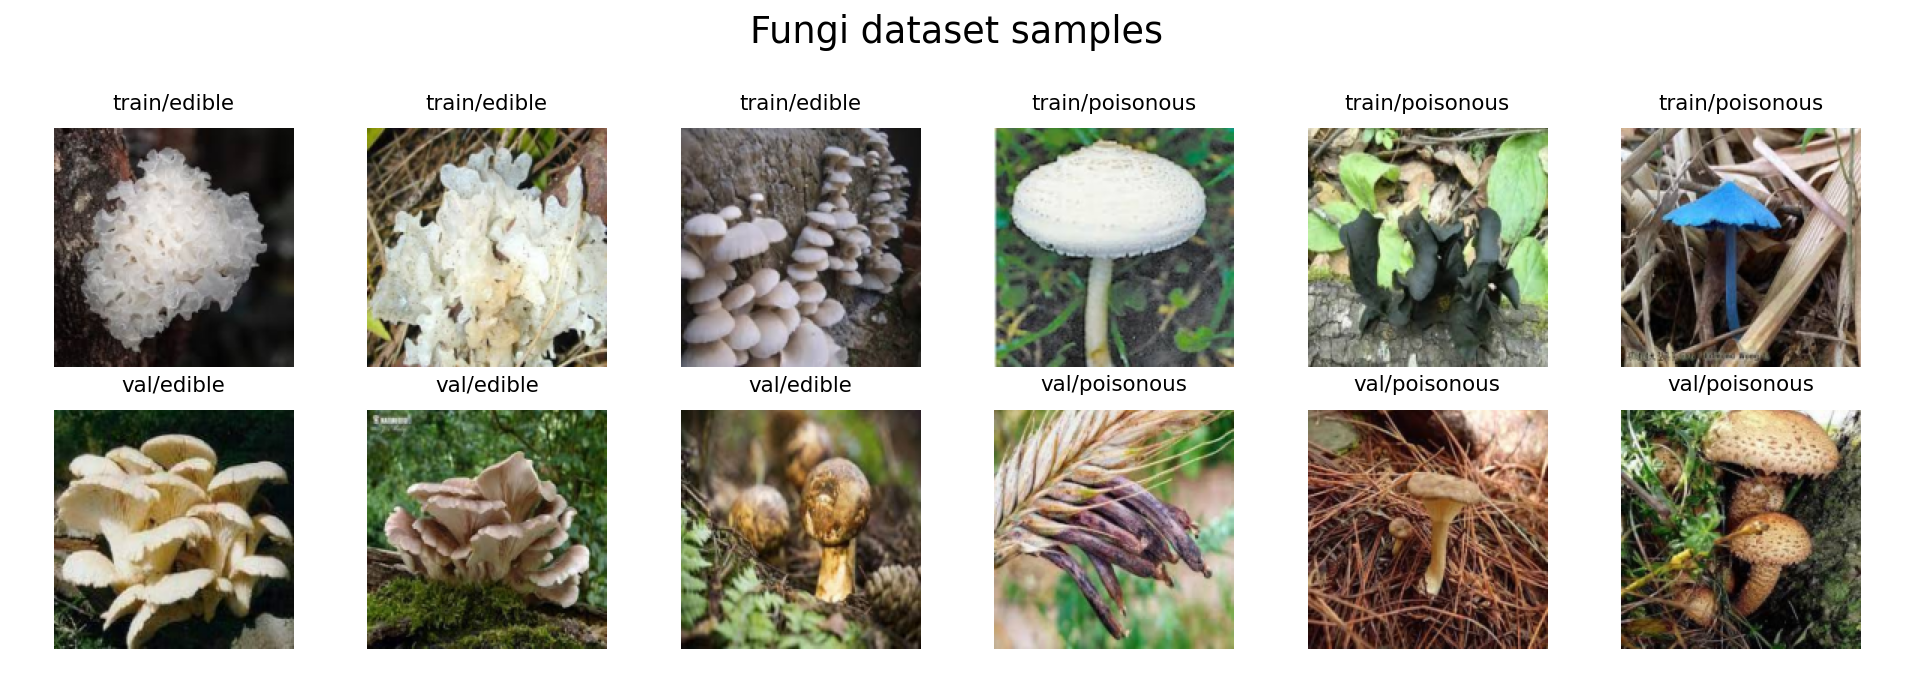
\includegraphics[width=\columnwidth]{fungi_dataset_samples.png}
\caption{Sample images from the fungi dataset. The word ``poisonous'' denotes the biological class label, not a poisoned training sample. The code uses lazy loading through a PyTorch \textit{Dataset}; images are not stacked into memory before batching.}
\label{fig:samples}
\end{figure}

%\subsection{Model Families and Architecture Hypotheses}


\subsection{The Periodic Table}

Let \(D=\{(x_i,y_i)\}_{i=1}^{n}\) be a clean training set and let \(\theta^\star(D)\) be the model trained by minimizing empirical loss. Poisoning replaces \(D\) with \(D'=D_{\mathrm{clean}}\cup D_{\mathrm{poison}}\). A general poisoning objective is
\begin{equation}
\begin{aligned}
 \max_{D_{\mathrm{poison}}\in\mathcal{C}}\quad
   & \mathcal{A}(\theta^\star(D_{\mathrm{clean}}\cup D_{\mathrm{poison}}))
   - c(D_{\mathrm{poison}})\\
 \text{s.t.}\quad
   & \theta^\star=\arg\min_{\theta}\mathcal{L}(\theta;D_{\mathrm{clean}}\cup D_{\mathrm{poison}}),
\end{aligned}
\end{equation}
where \(\mathcal{A}\) is the attacker's objective and \(\mathcal{C}\) encodes access constraints. The table columns are mechanism families: minimal/structural (M), optimization-based (O), gradient-based (G), backdoor/trigger (B), distributed/federated (D), supply-chain (S), retrieval/RAG (R), generative (N), and preference or alignment-data poisoning (P). Related evasion methods use the analogous M, O, G, and U columns in a separate companion panel.

Operational danger is scored as
\begin{equation}
\mathrm{DangerScore}=I\times S\times G_s\times C,
\end{equation}
where \(I\) is impact, \(S\) is stealth, \(G_s\) is scalability, and \(C\) is attacker cost-efficiency. The subscript avoids confusing scalability with the gradient-family column \(G\). These variables are qualitative rubric scores in \(\{1,2,3,4,5\}\), not calibrated probabilities or continuous measurements. A score of 1 denotes low adversarial advantage on that axis, and 5 denotes maximum adversarial advantage. Scores are assigned from literature consensus, implementation behavior, and the operational threat model; the product is intended as a transparent ordinal triage device. The maximum possible score is \(5^4=625\). Risk levels are R1: 400--625, R2: 200--399, R3: 100--199, and R4: below 100. Tables~\ref{tab:periodicpoison},~\ref{tab:periodicpoisonsystem}, and~\ref{tab:periodicevasion} demonstrate the visual taxonomy.

\begin{table}[t]
\centering
\caption{Mendeleev-style table, block A: learning-mechanism poisoning families. }
\label{tab:periodicpoison}
% Wrap the tabular in resizebox to force it to column width
\resizebox{\columnwidth}{!}{%
\begin{tabular}{@{}c c c c c c@{}}
\toprule
Risk & I. Minimal & II. Optimization & III. Gradient & IV. Backdoor & V. Distributed \\
\midrule
R1 & \btile & \ptile{ptO}{Fc}{Feature collision}{R1/O} & \btile & \ptile{ptB}{Wa}{WaNet}{R1/B} & \ptile{ptD}{Fl}{Fed replace}{R1/D} \\
R1 & \btile & \btile & \btile & \ptile{ptB}{Sa}{Sleeper agent}{R1/B} & \ptile{ptD}{Db}{DBA}{R1/D} \\
R1 & \btile & \btile & \btile & \ptile{ptB}{Cl}{Clean-label BD}{R1/B} & \btile \\
\midrule
R2 & \ptile{ptM}{Sp}{Subpopulation}{R2/M} & \ptile{ptO}{Bp}{Bullseye poly}{R2/O} & \ptile{ptG}{Wb}{Witches Brew}{R2/G} & \ptile{ptB}{Bn}{BadNets}{R2/B} & \ptile{ptD}{Al}{ALIE}{R2/D} \\
R2 & \ptile{ptM}{Cf}{Collab filter}{R2/M} & \ptile{ptO}{If}{Influence}{R2/O} & \btile & \ptile{ptB}{Hb}{Hidden BD}{R2/B} & \btile \\
R2 & \btile & \ptile{ptO}{Hp}{Hessian}{R2/O} & \btile & \ptile{ptB}{Ip}{Input-aware}{R2/B} & \btile \\
R2 & \btile & \ptile{ptO}{Cp}{Curriculum}{R2/O} & \btile & \ptile{ptB}{Nl}{NLP trigger}{R2/B} & \btile \\
\midrule
R3 & \ptile{ptM}{Tf}{Target flip}{R3/M} & \btile & \btile & \btile & \btile \\
R3 & \ptile{ptM}{Ko}{KNN poison}{R3/M} & \btile & \btile & \btile & \btile \\
R3 & \ptile{ptM}{Ts}{Time-series}{R3/M} & \btile & \btile & \btile & \btile \\
\midrule
R4 & \ptile{ptM}{Lf}{Random flip}{R4/M} & \ptile{ptO}{Svm}{SVM poison}{R4/O} & \btile & \btile & \btile \\
R4 & \ptile{ptM}{Oo}{Outlier}{R4/M} & \ptile{ptO}{RgN}{Regression}{R4/O} & \btile & \btile & \btile \\
\bottomrule
\end{tabular}%
} % end resizebox
\end{table}

\begin{table}[t]
\centering
\caption{Readable Mendeleev-style table, block B: system, retrieval, generative, and alignment-data poisoning families.}
\label{tab:periodicpoisonsystem}
\setlength{\tabcolsep}{3pt}
\renewcommand{\arraystretch}{1.05}
% Wrap the tabular in resizebox to force it to column width
\resizebox{\columnwidth}{!}{%
\begin{tabular}{@{}c c c c c@{}}
\toprule
Risk & VI. Supply & VII. Retrieval/RAG & VIII. Generative & IX. Preference/RLHF \\
\midrule
R1 & \ptile{ptS}{Ss}{Split-view}{R1/S} & \ptile{ptR}{Sd}{Single-doc RAG}{R1/R} & \ptile{ptN}{Ns}{Nightshade}{R1/N} & \btile \\
R1 & \ptile{ptS}{Fr}{Frontrun web}{R1/S} & \ptile{ptR}{Rg}{RAG poison}{R1/R} & \btile & \btile \\
\midrule
R2 & \btile & \ptile{ptR}{Gg}{Gradient RAG}{R2/R} & \ptile{ptN}{Td}{TrojDiff}{R2/N} & \ptile{ptP}{Bv}{Best-of-Venom}{R2/P} \\
R2 & \btile & \btile & \btile & \ptile{ptP}{Rl}{RLHF backdoor}{R2/P} \\
\midrule
R3 & \btile & \btile & \ptile{ptN}{Gd}{Glaze cloak}{R3/N} & \ptile{ptP}{Dp}{DPO poison}{R3/P} \\
R3 & \btile & \btile & \btile & \ptile{ptP}{Rp}{Reward poison}{R3/P} \\
\midrule
R4 & \btile & \btile & \btile & \btile \\
\bottomrule
\end{tabular}%
} % end resizebox
\end{table}
\begin{table}[t]
\centering
\caption{Readable Mendeleev-style companion table: related adversarial/evasion analogs included for comparison, not counted as data poisoning proper.}
\label{tab:periodicevasion}
\setlength{\tabcolsep}{3pt}
\renewcommand{\arraystretch}{1.05}
% Wrap the tabular in resizebox to force it to column width
\resizebox{\columnwidth}{!}{%
\begin{tabular}{@{}c c c c c@{}}
\toprule
Risk & I. Minimal & II. Optimization & III. Gradient & IV. Universal/Transfer \\
\midrule
R2 & \btile & \ptile{ptO}{Cw}{Carlini-Wagner}{R2/O} & \ptile{ptG}{Pg}{PGD}{R2/G} & \ptile{ptU}{Ap}{Adv. patch}{R2/U} \\
R2 & \btile & \ptile{ptO}{Ead}{Elastic Net}{R2/O} & \btile & \ptile{ptU}{Uap}{Universal pert.}{R2/U} \\
R2 & \btile & \btile & \btile & \ptile{ptU}{Eot}{EOT}{R2/U} \\
R2 & \btile & \btile & \btile & \ptile{ptU}{St}{Surrogate}{R2/U} \\
\midrule
R3 & \ptile{ptM}{Js}{JSMA}{R3/M} & \ptile{ptO}{Zo}{ZOO}{R3/O} & \ptile{ptG}{Fg}{FGSM}{R3/G} & \btile \\
R3 & \ptile{ptM}{Df}{DeepFool}{R3/M} & \ptile{ptO}{Bd}{Boundary}{R3/O} & \btile & \btile \\
\midrule
R4 & \ptile{ptM}{Sf}{SparseFool}{R4/M} & \btile & \btile & \btile \\
R4 & \ptile{ptM}{Op}{One-Pixel}{R4/M} & \btile & \btile & \btile \\
\bottomrule
\end{tabular}%
} % end resizebox
\end{table}
The layout keeps the Mendeleev-like table feel while avoiding literal chemical-table geometry: a tile's row is computed directly from the printed R label, so no R1 item can appear in an R2/R3 row. Inference-time evasion analogs are separated from poisoning attacks. Split-view web, frontend web, and single-document RAG entries are treated as data-source poisoning because they corrupt material later consumed by training, retrieval, or agent context rather than classic fixed training-set rows. Collaborative filtering poisoning is represented as sparse profile-injection or shilling. Glaze is retained as a defensive poisoning-like cloak, not as an ordinary malicious poisoning attack. Numbers are reference identifiers only, not chronology or severity ranking.


\subsection{Experimental Design}

Although the proposed table covers LLM, RAG, federated, generative, supply-chain, and preference/alignment poisoning, the empirical validation in this paper is scoped to computer-vision classification only.  Vision tasks provide visually auditable examples, fixed labels, explicit perturbation footprints, and a controlled setting in which training-time poisoning can be separated cleanly from inference-time evasion. The experiments, therefore, validate the metric logic and implementation discipline on a concrete subset of the taxonomy; they do not claim to empirically exhaust the RAG, RLHF, federated, or generative-system columns. Extending the benchmark suite to those threat models is reserved for future work.


\subsection{Model and Metrics}
 The study uses MobileNetV3-Small as a practical, lightweight transfer-learning baseline suitable for reduced-budget food-image pilot runs~\cite{mobilenetv3}. MobileNetV3-Small is a lightweight convolutional network built from mobile inverted bottleneck blocks, depthwise separable convolutions, squeeze-and-excitation modules, and hard-swish/ReLU nonlinearities. In our case, the original ImageNet classifier is removed. The frozen \texttt{features} stack maps each normalized RGB image to a 576-channel final convolutional representation; adaptive average pooling converts this tensor to a 576-dimensional embedding; and the trainable head is \(\mathrm{Dropout}(0.20)\) followed by a linear layer of size \(576\times C\), where \(C\) is the number of dataset classes.

The same architecture is used for clean baselines and poisoned retraining rows. For each poisoning method, a fresh classifier is trained on the modified training set under the same preprocessing and optimization settings; for evasion analogs, the attack is applied to the already trained clean baseline. The feature extractor is frozen in the reported runs, so Poison Frogs and Witches' Brew-style methods operate against a realistic transfer-learning threat model in which poisons mainly influence the classifier head and decision boundary. Images are resized to \(160\times160\) RGB for fungi and fish, while the reduced-budget seafood pilot uses \(96\times96\) RGB to keep the full method table executable locally.

This is explicitly a transfer-learning, or linear-probing, threat model. Let \(z=f_\phi(x)\) denote the MobileNetV3 feature vector and \(g_w(z)\) denote the newly initialized classifier head. When \(f_\phi\) is in \texttt{eval()} mode and all backbone parameters have \texttt{requires\_grad=False}, \(z\) is deterministic for a fixed image. Therefore, caching \(z\) and optimizing \(g_w\) is mathematically equivalent to repeatedly forwarding the same images through the frozen backbone and training only the head. We use this equivalence to make repeated poisoned retraining feasible on one workstation. The trade-off is scope: the experiments demonstrate poisoning of the linear-probe classifier and its decision boundary, not corruption of the frozen deep representation itself. This is a lower-bound attacker model compared with full end-to-end poisoning, where the adversary could also alter deep feature extractors and representation geometry. In cached-feature runs, online spatial or brightness augmentation is not applied after caching. Query-intensive evasion analogs such as ZOO and Boundary/HopSkipJump are evaluated on a conditional subset.


For poisoning and backdoors, the model is retrained on modified training data and evaluated on clean validation data plus an attack-specific metric. For evasion, success is conditional on the clean model first classifying the image correctly:
\begin{equation}
\mathrm{CSR}=
\frac{\sum_i \mathbf{1}[f(x_i)=y_i]\mathbf{1}[f(x_i')\neq y_i]}
{\sum_i \mathbf{1}[f(x_i)=y_i]}.
\label{eq:csr}
\end{equation}
This prevents inflated attack success caused by baseline errors. Table~\ref{tab:metrics} defines how normalized attack effect is interpreted for each attack type.



\begin{figure*}[t]
\centering
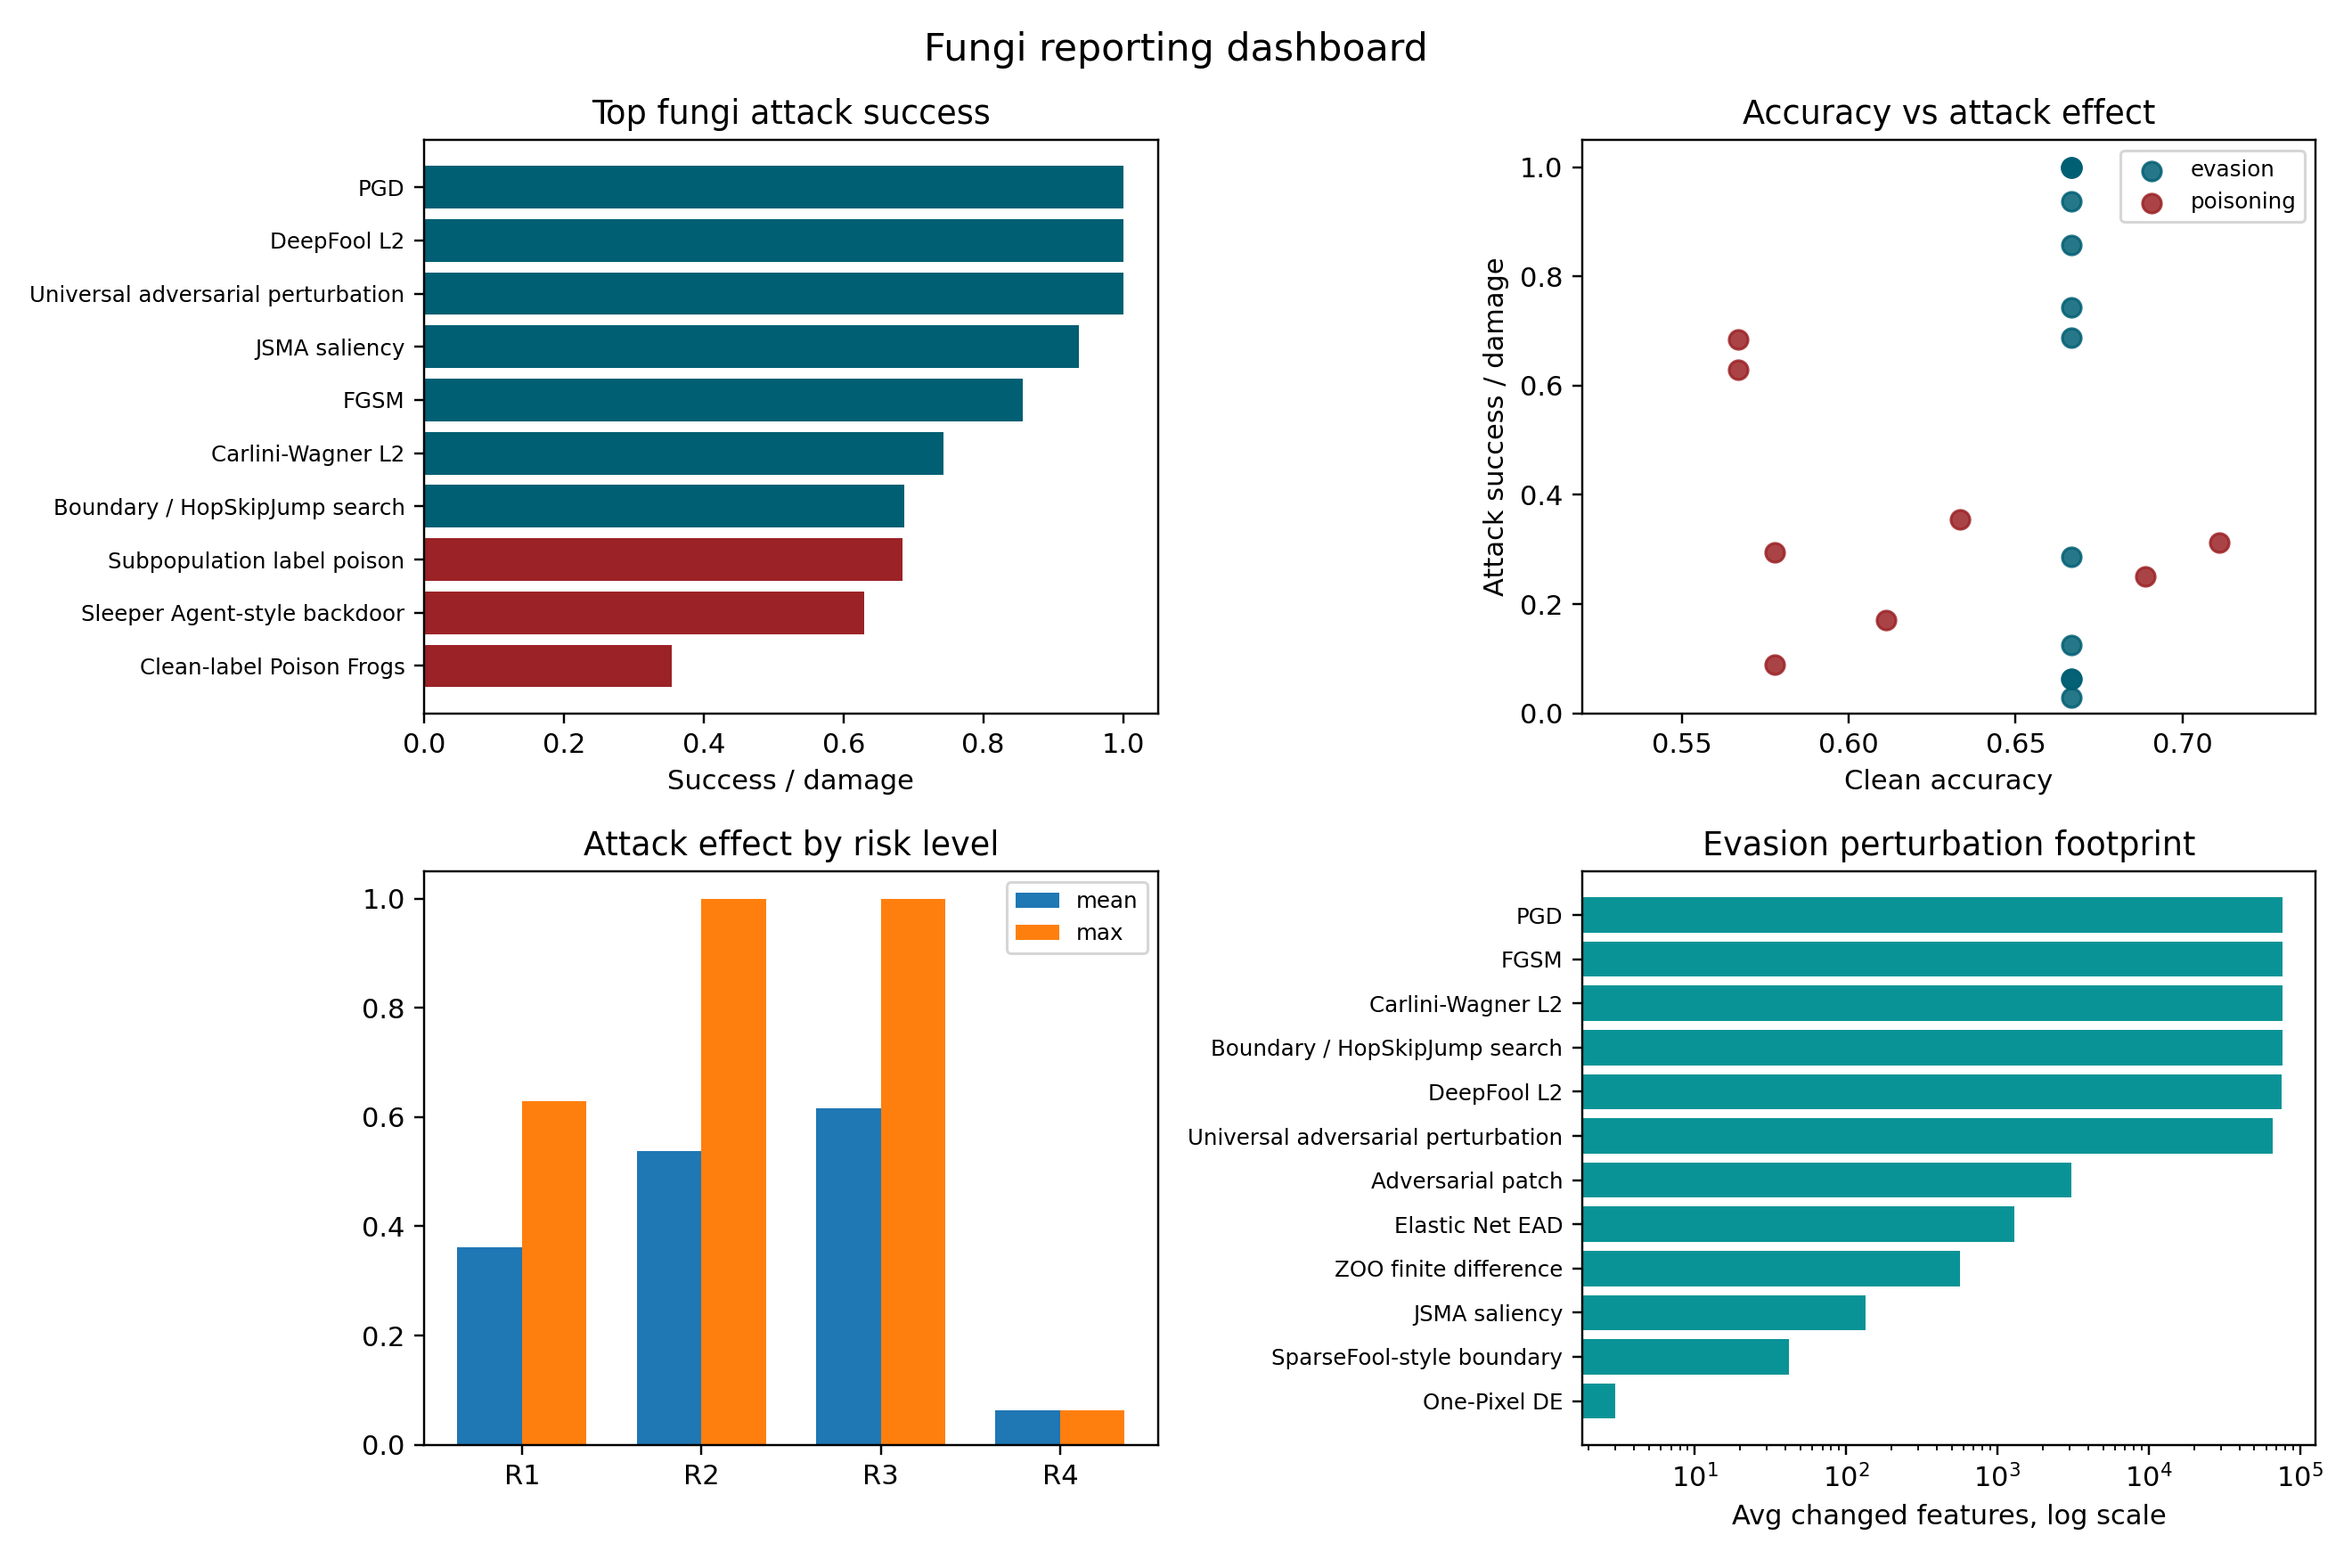
\includegraphics[width=0.92\textwidth]{fungi_reporting_dashboard.png}
\caption{Fungi reporting dashboard summarizing top attack/evasion effects, clean accuracy versus normalized attack-specific effect, effect by risk level, and evasion perturbation footprint measured as mean nonzero perturbed input dimensions.}
\label{fig:fungidashboard}
\end{figure*}

\begin{table}[t]
\centering
\caption{Stage-aware normalized attack-effect metrics.}
\label{tab:metrics}
\small
\begin{tabular}{p{0.23\columnwidth}p{0.39\columnwidth}p{0.23\columnwidth}}
\toprule
Attack type & Metric & Higher means \\
\midrule
Label flip or availability poison & Baseline accuracy minus attacked clean accuracy, clipped to \([0,1]\) & More global degradation \\
Targeted data poison & Target/source error rate or safety-critical confusion on clean validation data & Stronger targeted poisoning \\
Backdoor poison & Triggered test samples predicted as target label & Stronger trigger control \\
Clean-label poison & Target misclassification or critical confusion after retraining & Stronger clean-label effect \\
Evasion analog & Conditional success rate in Eq.~(\ref{eq:csr}) & Stronger inference-time failure \\
\bottomrule
\end{tabular}
\end{table}

%\subsection{Implementation Corrections}
 Clean-label Poison Frogs is implemented as latent feature optimization, minimizing feature distance while projecting the poison image back into an \(L_\infty\) ball around the base image. Other implemented methods include FGSM, PGD, DeepFool L2, Carlini-Wagner L2, Boundary/HopSkipJump search, One-Pixel differential evolution, and UAP. EAD uses a formal ISTA proximal solver: a gradient step on the smooth targeted objective followed by soft-thresholding for the \(L_1\) term and projection into the box and \(L_\infty\) constraints. JSMA saliency is vectorized across a batch. ZOO batches finite-difference coordinate probes. The adversarial patch is trained with random-location expectation over transformation.


%\subsection{Poisoning Results}
On fungi, the strongest poisoning-style selected-slice result is subpopulation poisoning, while the strongest trigger result is the gradient-aligned Sleeper-Agent-style backdoor. Poison Frogs increases the safety-critical poisonous-to-edible confusion above the clean baseline while preserving clean-label constraints. The Witches' Brew-style run demonstrates gradient alignment, but its measured effect is weaker on this small validation split than the subgroup and backdoor attacks.
 The clean seafood baseline reaches 1.0 accuracy with zero NonFresh-to-Fresh confusion. Under the reduced local attack budget, the strongest poisoning-style result is the Sleeper-Agent-style backdoor at 0.94 stealth-trigger ASR; BadNets reaches 0.5306 trigger ASR, while label/subpopulation poisoning produce small targeted effects and the current clean-label feature-collision and Witches' Brew-style pilots do not increase the safety-critical confusion.

%\subsection{Evasion Analog Stress Tests}

Evasion rows are reported as stress tests, not as evidence that those methods poison data. On fungi, PGD, DeepFool, and UAP reach 1.0 conditional untargeted success. These values are conditional on the clean-correct subset and therefore should be read with the sample count and baseline accuracy, not as a claim that the whole validation set is perfectly vulnerable. JSMA remains a strong sparse targeted method at 0.9375, while Carlini-Wagner reaches 0.7429 targeted ASR. On fish, FGSM, PGD, DeepFool, Carlini-Wagner, and UAP reach 1.0 conditional success, while EAD and Boundary/HopSkipJump reach 0.8 targeted ASR. On seafood, FGSM, PGD, DeepFool, Carlini-Wagner, EAD, UAP, adversarial patch, and Boundary/HopSkipJump reach 1.0 conditional success; JSMA reaches 0.25, and One-Pixel, SparseFool-style, and ZOO do not succeed in the reduced pilot budget. The full method-level rows, split plots, examples, and artifact inventory are retained in the GitHub supplement~\cite{KumarDataPoisonTable2026}.
\begin{table}[t]
\centering
\caption{Food-image dataset comparison.}
\label{tab:foodcomparison}
\small
\begin{tabular}{lrrrr}
\toprule
Dataset & Train & Clean & Top poison & Top evasion \\
\midrule
Fungi & 360 & 0.6667 & 0.6842 & 1.0 \\
Fish & 30 & 0.8 & 0.8 & 1.0 \\
Seafood & 300 & 1.0 & 0.9400 & 1.0 \\
\bottomrule
\end{tabular}
\end{table}






\section{Conclusion}
We structure our conclusion as answers to the study Research Questions.
\textbf{RQ1:} The table answers the organization question by making every coordinate auditable: the vertical coordinate is the assigned R1, R2, R3, or R4 level; the horizontal coordinate is the mechanism family; and the panel determines whether a method is poisoning proper or an evasion/transfer analog. This removes arbitrary chemical-table gaps, prevents a cell labeled R1 from appearing in an R2 or R3 row, and separates related evasion methods from data-poisoning methods.
\textbf{RQ2:} On the fungi pilot task, the largest evasion stress-test failures are PGD, DeepFool, and UAP with 1.0 conditional untargeted success; JSMA reaches 0.9375 conditional targeted ASR and Carlini-Wagner reaches 0.7429. On the fish micro-batch proof of concept, FGSM, PGD, DeepFool, Carlini-Wagner, and UAP reach 5/5 conditional success, while the Sleeper-Agent-style backdoor reaches 4/5 stealth-trigger ASR. These fish values demonstrate code-path coverage and a safety-critical direction on a tiny specialty dataset, not a robust estimate. On the seafood replacement benchmark, the clean baseline reaches 1.0 accuracy; the strongest poisoning-style result is the Sleeper-Agent-style backdoor at 0.9400 stealth-trigger ASR, and the strongest evasion stress tests again reach 1.0 conditional success. These results answer RQ2 by showing that inference-time methods can be strongest under conditional evaluation, while subgroup and backdoor poisoning create the most important training-time targeted failures.
\textbf{RQ3:} The experiment answers the implementation question by replacing in-memory image stacking with lazy loading, replacing a weak from-scratch CNN with pretrained MobileNetV3-Small transfer learning, using true latent-space feature collision instead of pixel blending, adding explicit poster-method implementations, vectorizing JSMA, batching ZOO finite-difference queries, reporting conditional attack success only on clean-correct examples, and disclosing seeds plus the repeated-run protocol required for journal submission.

%\section{Discussion}

%The results support three security lessons. First, aggregate accuracy is not a sufficient safety metric. The clean fungi baseline already confuses some poisonous samples as edible, and several attacks worsen a targeted failure mode without simply maximizing visible accuracy collapse; because the baseline is only 0.6667 accurate, fungi attack effects are interpreted as stress-test evidence rather than a mature production classifier result. Second, attack stage matters. Evasion methods can be dramatic, but they should not be described as poisoning unless they enter the training or adaptation data. Third, realistic baselines matter: pretrained transfer learning, lazy loading, hierarchical folder labeling, and conditional success metrics make the food-image experiments closer to an operational AI safety presentation than a purely toy implementation. The seafood replacement benchmark is useful because it has a stronger clean baseline, but it remains a reduced-budget pilot: the current clean-label feature-collision and Witches' Brew-style variants are reported as negative targeted-confusion results rather than hidden or overclaimed.

%The implementation audit is intentionally conservative. The code reproduces the core mechanism of all poster methods plus ten additional shared methods: Poison Frogs, Sleeper-Agent-style backdoor, Adversarial Patch, Witches' Brew-style gradient matching, JSMA, ZOO, SparseFool-style sparse boundary search, EAD, subpopulation poisoning, and BadNets. It does not claim industrial-scale transferability, full physical-world patch robustness, or long-horizon LLM sleeper-agent persistence.

%\subsection{Synthesis from Taxonomy Elicitation}

%The extended candidate lists used while building the table are useful as elicitation material, but they are not treated as primary literature evidence. Their value is that many independent descriptions converged on the same operational themes. First, the highest-risk poisoning entries tend to be stealth-preserving: clean-label feature collision, bullseye/polytope variants, clean-label backdoors, and gradient-matching poisons all aim to avoid obvious label errors while moving the model in feature or gradient space. Second, trigger attacks form a spectrum from visible patch backdoors to hidden, semantic, augmentation-stable, or sleeper-style triggers; the common defense failure is that clean validation accuracy can remain high while triggered behavior is uncontrolled. Third, universal and transfer attacks, including adversarial patches, UAP, EOT, and surrogate-transfer attacks, are best interpreted as stress tests unless their artifacts are inserted into training or retrieval data. Fourth, minimal attacks such as label flipping, KNN/geometric poisoning, JSMA, One-Pixel, and SparseFool are valuable because they reveal how little structural change may be needed, but their operational risk depends strongly on scale, access, and detectability.

%The elicitation also exposed taxonomy pressure points that shaped the final table. Some methods can reasonably fit more than one mechanism column: Poison Frogs can be described as optimization-based, gradient-assisted, or feature-space minimal depending on the implementation; adversarial patch can be localized/minimal in geometry but universal in reuse; and influence-function attacks are optimization attacks that rely on first- or second-order gradient information. Rather than forcing a single universal truth, the table assigns the mechanism that is most useful for the threat model and explains implementation fidelity in Table~\ref{tab:fidelity}. The strongest future extension is an ecosystem-stage axis: pretraining poisoning, fine-tuning poisoning, federated/update poisoning, retrieval poisoning, preference/alignment poisoning, and inference-time evasion have different defenders, observability, and recovery options even when their mathematics look similar.


%\section{Limitations}

%Several limitations matter before journal submission. First, the empirical benchmark is vision-only. The taxonomy covers RAG, RLHF/preference, federated, generative, and supply-chain attacks, but the executed experiments are limited to controlled image classification so that labels, triggers, perturbation footprints, and poisoning-versus-evasion distinctions are auditable. Second, the fish dataset is very small: only 40 images total and 10 validation images after the deterministic split. Fish results are therefore a few-shot micro-batch proof of concept and implementation check, not statistically powered estimates. The apparent ``healing'' in some fish poisoning rows, where clean accuracy rises from 8/10 to 10/10, is a warning sign of tiny-split variance and overfitting rather than evidence that poisoning regularizes the model. The wall of 0/5 attack metrics for several fish poisoning rows is also a negative hyperparameter-transfer result: those settings were not tuned for a 30-image MobileNetV3 fine-tuning regime. Third, the fungi baseline accuracy is modest at 0.6667, which means attack effects must be interpreted alongside baseline instability and clean-correct conditional metrics. Fourth, the seafood replacement benchmark is larger and cleaner than the fish pilot, but the reported run still uses \(96\times96\) images, two training epochs, and \texttt{attack\_scale=0.12}; full-budget attacks and repeated seeds are needed before journal claims. Fifth, the current food-image artifact set reports deterministic single-seed pilot runs. A journal version should execute the seed sets in Table~\ref{tab:seeds}, report mean \(\pm\) standard deviation for every metric, and regenerate all bar plots with seed-level error bars. Sixth, frozen-feature caching is a linear-probing optimization, not an unrestricted full-network poisoning benchmark: it improves computational feasibility but removes fresh per-epoch augmentation unless augmented views are cached and restricts claims to classifier-head poisoning. Seventh, several implemented attacks are explicitly style variants or approximations as documented in Table~\ref{tab:fidelity}. Eighth, the paper includes evasion analogs for stress testing and comparison, but those methods are not counted as data poisoning proper unless their outputs enter a training, retrieval, or adaptation loop. Finally, the taxonomy includes literature-level entries for RAG, supply-chain, federated, generative, and alignment poisoning that are not all executed in the image experiments.

%\section{Conclusion}

This paper answers the three research questions as follows. First, data poisoning can be organized as an auditable risk-by-mechanism matrix by separating risk, mechanism, and poisoning-versus-evasion status. Second, the pilot fungi, fish, and seafood experiments show that PGD, DeepFool, UAP, JSMA, Carlini-Wagner, EAD, and patch-style attacks can produce the strongest evasion stress-test failures, while subpopulation poisoning and Sleeper-Agent-style backdoors produce the strongest training-time targeted failures in the reported food-image runs. Third, realistic conclusions require careful engineering: lazy loading, transfer learning, hierarchical dataset parsing, latent-space poisoning, explicit implementation coverage, vectorized/batched attacks, conditional success metrics, and repeated-seed reporting. The final framework is suitable for an at-a-glance AI security presentation, while a journal version should expand the food-image datasets and complete the repeated-run protocol.

\begin{thebibliography}{99}

\bibitem{mobilenetv3}
A. Howard et al., ``Searching for MobileNetV3,'' in \emph{Proc. IEEE/CVF International Conference on Computer Vision (ICCV)}, 2019, pp. 1314--1324. [Online]. Available: \url{https://openaccess.thecvf.com/content_ICCV_2019/html/Howard_Searching_for_MobileNetV3_ICCV_2019_paper.html}

\bibitem{adversaguard}
Y. Kumar, S. Thomas, D. Gayle, J. J. Li, and D. Kruger, ``AdversaGuard: A distributed data-poisoning benchmark for parallel AI,'' in \emph{SC25 Posters, The International Conference for High Performance Computing, Networking, Storage and Analysis}, 2025, 2 pages. [Online]. Available: \url{https://sc25.supercomputing.org/proceedings/posters/poster_files/post110s2-file3.pdf}

\bibitem{biggio2012}
B. Biggio, B. Nelson, and P. Laskov, ``Poisoning attacks against support vector machines,'' in \emph{Proc. International Conference on Machine Learning (ICML)}, 2012. [Online]. Available: \url{https://icml.cc/2012/papers/880.pdf}

\bibitem{mei2015}
S. Mei and X. Zhu, ``Using machine teaching to identify optimal training-set attacks on machine learners,'' in \emph{Proc. AAAI Conference on Artificial Intelligence}, vol. 29, no. 1, 2015, pp. 2871--2877, doi: 10.1609/aaai.v29i1.9569. [Online]. Available: \url{https://ojs.aaai.org/index.php/AAAI/article/view/9569}

\bibitem{badnets}
T. Gu, B. Dolan-Gavitt, and S. Garg, ``BadNets: Identifying vulnerabilities in the machine learning model supply chain,'' arXiv:1708.06733, 2017, doi: 10.48550/arXiv.1708.06733. [Online]. Available: \url{https://arxiv.org/abs/1708.06733}

\bibitem{targetedbackdoor}
X. Chen, C. Liu, B. Li, K. Lu, and D. Song, ``Targeted backdoor attacks on deep learning systems using data poisoning,'' arXiv:1712.05526, 2017, doi: 10.48550/arXiv.1712.05526. [Online]. Available: \url{https://arxiv.org/abs/1712.05526}

\bibitem{poisonfrogs}
A. Shafahi et al., ``Poison Frogs! Targeted clean-label poisoning attacks on neural networks,'' in \emph{Advances in Neural Information Processing Systems}, vol. 31, 2018. [Online]. Available: \url{https://papers.neurips.cc/paper_files/paper/2018/hash/22722a343513ed45f14905eb07621686-Abstract.html}

\bibitem{witchesbrew}
J. Geiping et al., ``Witches' Brew: Industrial scale data poisoning via gradient matching,'' arXiv:2009.02276, 2020, doi: 10.48550/arXiv.2009.02276. [Online]. Available: \url{https://arxiv.org/abs/2009.02276}

\bibitem{webscale}
N. Carlini et al., ``Poisoning web-scale training datasets is practical,'' arXiv:2302.10149, 2024, doi: 10.48550/arXiv.2302.10149. [Online]. Available: \url{https://arxiv.org/abs/2302.10149}

\bibitem{poisonedrag}
W. Zou, R. Geng, B. Wang, and J. Jia, ``PoisonedRAG: Knowledge corruption attacks to retrieval-augmented generation of large language models,'' arXiv:2402.07867, 2024, doi: 10.48550/arXiv.2402.07867. [Online]. Available: \url{https://arxiv.org/abs/2402.07867}

\bibitem{nightshade}
S. Shan et al., ``Nightshade: Prompt-specific poisoning attacks on text-to-image generative models,'' arXiv:2310.13828, 2023, doi: 10.48550/arXiv.2310.13828. [Online]. Available: \url{https://arxiv.org/abs/2310.13828}

\bibitem{goodfellow2014}
I. J. Goodfellow, J. Shlens, and C. Szegedy, ``Explaining and harnessing adversarial examples,'' arXiv:1412.6572, 2014. [Online]. Available: \url{https://arxiv.org/abs/1412.6572}

\bibitem{madry2017}
A. Madry, A. Makelov, L. Schmidt, D. Tsipras, and A. Vladu, ``Towards deep learning models resistant to adversarial attacks,'' arXiv:1706.06083, 2017. [Online]. Available: \url{https://arxiv.org/abs/1706.06083}

\bibitem{deepfool}
S.-M. Moosavi-Dezfooli, A. Fawzi, and P. Frossard, ``DeepFool: a simple and accurate method to fool deep neural networks,'' in \emph{Proc. IEEE Conference on Computer Vision and Pattern Recognition (CVPR)}, 2016. [Online]. Available: \url{https://arxiv.org/abs/1511.04599}

\bibitem{cw}
N. Carlini and D. Wagner, ``Towards evaluating the robustness of neural networks,'' in \emph{Proc. IEEE Symposium on Security and Privacy}, 2017, doi: 10.1109/SP.2017.49. [Online]. Available: \url{https://arxiv.org/abs/1608.04644}

\bibitem{onepixel}
J. Su, D. V. Vargas, and K. Sakurai, ``One pixel attack for fooling deep neural networks,'' \emph{IEEE Transactions on Evolutionary Computation}, vol. 23, no. 5, pp. 828--841, 2019, doi: 10.1109/TEVC.2019.2890858. [Online]. Available: \url{https://arxiv.org/abs/1710.08864}

\bibitem{uap}
S.-M. Moosavi-Dezfooli, A. Fawzi, O. Fawzi, and P. Frossard, ``Universal adversarial perturbations,'' in \emph{Proc. IEEE Conference on Computer Vision and Pattern Recognition (CVPR)}, 2017. [Online]. Available: \url{https://arxiv.org/abs/1610.08401}

\bibitem{jsma}
N. Papernot, P. McDaniel, S. Jha, M. Fredrikson, Z. B. Celik, and A. Swami, ``The limitations of deep learning in adversarial settings,'' in \emph{Proc. IEEE European Symposium on Security and Privacy (EuroS\&P)}, 2016, pp. 372--387, doi: 10.1109/EuroSP.2016.36. [Online]. Available: \url{https://doi.org/10.1109/EuroSP.2016.36}

\bibitem{ead}
P.-Y. Chen, Y. Sharma, H. Zhang, J. Yi, and C.-J. Hsieh, ``EAD: Elastic-net attacks to deep neural networks via adversarial examples,'' in \emph{Proc. AAAI Conference on Artificial Intelligence}, 2018. [Online]. Available: \url{https://arxiv.org/abs/1709.04114}

\bibitem{zoo}
P.-Y. Chen, H. Zhang, Y. Sharma, J. Yi, and C.-J. Hsieh, ``ZOO: Zeroth order optimization based black-box attacks to deep neural networks without training substitute models,'' in \emph{Proc. ACM Workshop on Artificial Intelligence and Security}, 2017, doi: 10.1145/3128572.3140448. [Online]. Available: \url{https://arxiv.org/abs/1708.03999}

\bibitem{boundaryattack}
W. Brendel, J. Rauber, and M. Bethge, ``Decision-based adversarial attacks: Reliable attacks against black-box machine learning models,'' in \emph{Proc. International Conference on Learning Representations (ICLR)}, 2018. [Online]. Available: \url{https://arxiv.org/abs/1712.04248}

\bibitem{hopskipjump}
J. Chen, M. I. Jordan, and M. J. Wainwright, ``HopSkipJumpAttack: A query-efficient decision-based attack,'' in \emph{Proc. IEEE Symposium on Security and Privacy}, 2020. [Online]. Available: \url{https://arxiv.org/abs/1904.02144}

\bibitem{adversarialpatch}
T. B. Brown, D. Mane, A. Roy, M. Abadi, and J. Gilmer, ``Adversarial patch,'' arXiv:1712.09665, 2017, doi: 10.48550/arXiv.1712.09665. [Online]. Available: \url{https://arxiv.org/abs/1712.09665}

\bibitem{sparsefool}
A. Modas, S.-M. Moosavi-Dezfooli, and P. Frossard, ``SparseFool: a few pixels make a big difference,'' in \emph{Proc. IEEE/CVF Conference on Computer Vision and Pattern Recognition (CVPR)}, 2019. [Online]. Available: \url{https://arxiv.org/abs/1811.02248}

\bibitem{agustyawan2020fish}
A. Agustyawan, ``Fresh and not fresh fish dataset,'' Kaggle dataset, 2020. [Online]. Available: \url{https://www.kaggle.com/datasets/arifagustyawan/fresh-and-not-fresh-fish-dataset/data}

\bibitem{ulucan2020fish}
O. Ulucan, D. Karakaya, and M. Turkan, ``A large-scale dataset for fish segmentation and classification,'' in \emph{Proc. Innovations in Intelligent Systems and Applications Conference (ASYU)}, 2020, pp. 1--5, doi: 10.1109/ASYU50717.2020.9259867. [Online]. Available: \url{https://www.kaggle.com/datasets/crowww/a-large-scale-fish-dataset}

\bibitem{KumarDataPoisonTable2026}
Y.~Kumar, ``datapoisontable: Data Poisoning Risk Matrix and experimental artifacts,'' GitHub repository, 2026. [Online]. Available: \url{https://github.com/ykumar2020/datapoisontable}. Accessed: May 10, 2026.
\end{thebibliography}


\end{document}
